\documentclass[10pt,a4paper,final]{article} %draft

\usepackage[english, russian]{babel}

\usepackage{geometry}
%\usepackage[a4paper,left=2cm,right=2cm,top=2cm,bottom=2cm,bindingo ffset=0cm]{geometry}

\usepackage[utf8]{inputenc}

\usepackage[final]{pdfpages}

\usepackage{textcomp,enumitem}

\usepackage{amsmath,amsthm,amssymb}

\usepackage{booktabs}

\usepackage{listings}
\usepackage{xcolor}
\usepackage{caption}
\usepackage{adjustbox}


\definecolor{codegray}{rgb}{0.95,0.95,0.95}
\definecolor{codepurple}{rgb}{0.58,0,0.82}
\definecolor{codegreen}{rgb}{0,0.5,0} % зеленый цвет
\definecolor{codeblue}{rgb}{0,0,0.5} % синий цвет
\definecolor{codestring}{rgb}{0.64,0.08,0.08} % цвет строк


\lstset{
	language=C++,
	extendedchars=true,
	literate=
	{а}{{\selectfont\char224}}1
	{б}{{\selectfont\char225}}1
	{в}{{\selectfont\char226}}1
	{г}{{\selectfont\char227}}1
	{д}{{\selectfont\char228}}1
	{е}{{\selectfont\char229}}1
	{ж}{{\selectfont\char230}}1
	{з}{{\selectfont\char231}}1
	{и}{{\selectfont\char232}}1
	{й}{{\selectfont\char233}}1
	{к}{{\selectfont\char234}}1
	{л}{{\selectfont\char235}}1
	{м}{{\selectfont\char236}}1
	{н}{{\selectfont\char237}}1
	{о}{{\selectfont\char238}}1
	{п}{{\selectfont\char239}}1
	{р}{{\selectfont\char240}}1
	{с}{{\selectfont\char241}}1
	{т}{{\selectfont\char242}}1
	{у}{{\selectfont\char243}}1
	{ф}{{\selectfont\char244}}1
	{х}{{\selectfont\char245}}1
	{ц}{{\selectfont\char246}}1
	{ч}{{\selectfont\char247}}1
	{ш}{{\selectfont\char248}}1
	{щ}{{\selectfont\char249}}1
	{ъ}{{\selectfont\char250}}1
	{ы}{{\selectfont\char251}}1
	{ь}{{\selectfont\char252}}1
	{э}{{\selectfont\char253}}1
	{ю}{{\selectfont\char254}}1
	{я}{{\selectfont\char255}}1
	{А}{{\selectfont\char192}}1
	{Б}{{\selectfont\char193}}1
	{В}{{\selectfont\char194}}1
	{Г}{{\selectfont\char195}}1
	{Д}{{\selectfont\char196}}1
	{Е}{{\selectfont\char197}}1
	{Ж}{{\selectfont\char198}}1
	{З}{{\selectfont\char199}}1
	{И}{{\selectfont\char200}}1
	{Й}{{\selectfont\char201}}1
	{К}{{\selectfont\char202}}1
	{Л}{{\selectfont\char203}}1
	{М}{{\selectfont\char204}}1
	{Н}{{\selectfont\char205}}1
	{О}{{\selectfont\char206}}1
	{П}{{\selectfont\char207}}1
	{Р}{{\selectfont\char208}}1
	{С}{{\selectfont\char209}}1
	{Т}{{\selectfont\char210}}1
	{У}{{\selectfont\char211}}1
	{Ф}{{\selectfont\char212}}1
	{Х}{{\selectfont\char213}}1
	{Ц}{{\selectfont\char214}}1
	{Ч}{{\selectfont\char215}}1
	{Ш}{{\selectfont\char216}}1
	{Щ}{{\selectfont\char217}}1
	{Ъ}{{\selectfont\char218}}1
	{Ы}{{\selectfont\char219}}1
	{Ь}{{\selectfont\char220}}1
	{Э}{{\selectfont\char221}}1
	{Ю}{{\selectfont\char222}}1
	{Я}{{\selectfont\char223}}1,
	%	{|}{{\textbar}}1,
	%	{||}{{\textbar\textbar}}1
	%	{\&}{{\string&}}1
	%	{==}{{\string==}}1
	%	{\string\\}{{\string\\}}1,
	numbers=left,
	stepnumber=1,
	firstnumber=1,
	numberstyle=\tiny,
	basicstyle=\ttfamily\footnotesize,
	breakatwhitespace=false,
	breaklines=true,
	captionpos=b,
	keepspaces=true,
	showspaces=false,
	showstringspaces=false,
	showtabs=false,
	tabsize=2,
	frame=single,
	keywordstyle=\color{codeblue}, % ключевые слова
	commentstyle=\color{codegreen}, % комментарии
	stringstyle=\color{codestring}, % строки
	%identifierstyle=\color{green}, % стиль для переменных
	backgroundcolor=\color{codegray},
}
%\usepackage{fancyvrb}

%\usepackage{fancyhdr}

%\usepackage{upgreek}

%\usepackage{tipa}

%\usepackage{tikz}

%\usepackage{graphicx}

%\usepackage{pgfplots}

\usepackage{indentfirst}

%\usepackage{gensymb}

%\usepackage{amssymb}

%\usepackage{pdfpages}

\usepackage[unicode, pdftex, colorlinks, urlcolor=blue]{hyperref}

%\usepackage[T2A]{fontenc}


\usepackage{tabularx}
\usepackage{multirow}


\usepackage{graphics}

\linespread{1.5}

\pagestyle{plain}

%\usepackage{listings} 
%\usepackage{moreverb} 

%\setlist[enumerate,itemize]{leftmargin=1.2cm} %отступ в перечислениях

\hypersetup{
	colorlinks=true,
	linkcolor=black,
	%allcolors=[RGB]{0 0 0}}
	}
	%\lstloadlanguages{ [LaTeX] TeX}
	
	\lstloadlanguages{ [LaTeX] TeX}
	
	
	
	\textheight=24cm 
	\textwidth=16cm
	\oddsidemargin=0pt 
	\topmargin=-1.5cm
	\parindent=24pt 
	\parskip=0pt 
	\tolerance=2000 
	\flushbottom 
	
	%\usepackage[font=scriptsize]{caption}
	\usepackage[labelsep=period]{caption}
	
	
	\usepackage{tocloft}
	
	\setlength{\cftbeforesecskip}{0.3ex}   % Расстояние перед секцией
	\setlength{\cftbeforesubsecskip}{0.1ex} % Расстояние перед подразделом
	\setlength{\cftbeforesubsubsecskip}{0.1ex} % Расстояние перед под-подразделом
	
	\begin{document}
\thispagestyle{empty}

\begin{center}
	{\Large МИНОБРНАУКИ РОССИИ}\\
	~\\
	{\large ФЕДЕРАЛЬНОЕ ГОСУДАРСТВЕННОЕ БЮДЖЕТНОЕ ОБРАЗОВАТЕЛЬНОЕ УЧРЕЖДЕНИЕ ВЫСШЕГО ПРОФЕССИОНАЛЬНОГО ОБРАЗОВАНИЯ}\\
	~\\
	{\Large \bf <<САНКТ-ПЕТЕРБУРГСКИЙ ПОЛИТЕХНИЧЕСКИЙ УНИВЕРСИТЕТ ПЕТРА ВЕЛИКОГО>>}\\
	~\\
	{\large Институт компьютерных наук и кибербезопасности}\\
	{\large Высшая школа технологий искусственного интеллекта}\\
	{\large Направление 02.03.01 Математика и компьютерные науки}\\
	~\\
	~\\
	~\\
	~\\
	{\Large \bf Отчет по курсовой работе}\\
	{\Large по дисциплине <<Теория алгоритмов>> }\\
	~\\
	~\\
	
	{\Large Синтез функциональной схемы часов}\\
		{\large  Вариант № 22.}\\ 	
	
	~\\
	~\\
	~\\
	~\\
	~\\
	~\\
	~\\
	{\large Обучающийся: \underline{\hspace{3.5cm}} \qquad\qquad Гладков И.А.}\\
	~\\
	{\large Руководитель: \underline{\hspace{3.5cm}} \hspace{16mm} Востров А.В.}\\
	~\\
	~\\
\end{center}
\begin{flushright}
	
	«\underline{\hspace{1cm}}»\underline{\hspace{3cm}}20\underline{\hspace{0.7cm}}г.
\end{flushright}
~\\
\begin{center}
	{\large Санкт-Петербург, 2024}
\end{center}
\newpage

\tableofcontents

\newpage
\addcontentsline{toc}{section}{Введение}
\section*{Введение}
Данная курсовая работа представляет собой спроектированную схему, реализующую работу часов со следующими характеристиками:

\begin{itemize}
	\item Отображение и корректировка минут, часов.
	\item Отключение индикаторов с целью экономии электроэнергии.
	\item Останов часов после состояния корректировки текущего времени.
	\item Секундомер с фиксацией накопленного времени и возможностью продолжения отсчета секундомера.
	\item Звуковая сигнализация каждые четверть часа в течение секунды.
\end{itemize}


\newpage
\section{Постановка задач}
Необходимо построить функциональную схему электронных часов в соответствии с вариантом 22 (0112220):
\begin{itemize}
	\item Отображение и корректировка минут, часов.
	\item 24-x часовой режим работы часов.
	\item Отключение индикаторов с целью экономии электроэнергии.
	\item Останов часов после состояния корректировки текущего времени.
	\item Секундомер с фиксацией накопленного времени и возможностью продолжения отсчета секундомера.
	\item Звуковая сигнализация каждые четверть часа в течение секунды.
\end{itemize}

Для построения функциональной схемы часов требуется выполнить следующие этапы:
\begin{enumerate}
	\item Построить граф управляющего автомата часов и дать пояснения к нему.
	\item Изобразить общую структурную схему часов с указаниями всех необходимых управляющих.
	\item Закодировать входные и выходные воздействия, а также  состояния автомат.
	\item  Минимизировать функции блоков F и FL.
	\item Построить общую функциональную схему.
	\item Определить примерную площадь микросхемы, реализующей построенную функциональную схему при современной плотности компоновки транзисторов.
\end{enumerate}


\newpage
\section{Математическое описание}
\subsection{Конечный автомат}
Математическая модель дискретного устройства, которая описывается набором $A = (S, X, Z, s_0, \delta, \lambda)$, где 
\begin{itemize}
	\item $S = (s_0, s_1, s_2, ... , s_m) \text{-- множество состояний}$
	\item $X = (x_0, x_1, x_2, ... , x_m) \text{-- множество входных сигналов}$
	\item $Z = (y_0, y_1, y_2, ... , y_m) \text{-- множество выходных сигналов}$
	\item $s_0 \text{-- начальное состояние} $
	\item $\delta: S \times X \rightarrow S \text{-- функция переходов}$
	\item  $\lambda: S \times X \rightarrow Y \text{-- функция выходов}$
\end{itemize}

Конечный автомат работает в дискретные моменты времени. В момент времени $t=0$ автомат всегда будет находиться в начальном состоянии $s_0$.

\subsection{Реализация графа управляющего автомата часов}
\subsubsection{Граф управляющего автомата}
Граф управляющего конечного автомата электронных часов изображен на  \hyperref[КА]{рисунке 1}.
\newpage
\begin{figure}[htpb]
	\centering
	\includegraphics[scale=0.6]{img/КА.png}
	\label{КА} 
	\caption{Граф конечного автомата для часов}
\end{figure}

\subsubsection{Состояния конечного автомата}
Было выделено 7 состояний автомата: $$S = \{s_0, s_1, s_2, s_3, s_4, s_5, s_6\}$$
\begin{enumerate}[label=""]
	\item $s_0$: \textbf{time} -- состояние отображения текущего времени. На индикаторах отображаются значения часов и минут. При нажатии кнопки <<a>> происходит переход в состояние корректировки минут, при нажатии <<b>> -- переход в секундомер, при нажатии <<ab>> -- происходит переход в состояние экономии энергии.
	\item $s_1$: \textbf{minutes correction} -- состояние корректировки значения минут. На индикаторах отображается только значение минут. При нажатии кнопки <<a>> происходит переход в состояние корректировки часов, при нажатии <<b>> значение минут увеличивается на один, при нажатии <<ab>> ничего не происходит.
	\item $s_2$: \textbf{hours correction} -- состояние корректировки значения часов. На индикаторах отображается только значение часов. При нажатии кнопки <<a>> происходит переход в состояние останова времени часов, при нажатии <<b>> значение часов увеличивается на один, при нажатии <<ab>> ничего не происходит.
	\item $s_3$: \textbf{stop time} -- состояние останова часов. На индикаторах отображаются значения часов и минут, но время не идет.  При нажатии кнопки <<a>> происходит переход в состояние корректировки минут, при нажатии <<b>> переходит в состояние отображения времени, то есть время на часах продолжает идти, при нажатии <<ab>> ничего не происходит.
	\item $s_4$: \textbf{sec stop} -- состояние остановленного секундомера. На индикаторах -- минуты и секунды. По нажатию <<a>> запускается секундомер, <<b>> -- переход в отображение времени, <<ab>> -- сброс времени секундомера.
	\item $s_5$: \textbf{sec run} -- состояние работающего секундомера. На индикаторах -- минуты и секунды. По нажатию <<a>> секундомер останавливается, <<b>> -- переход в отображение времени (значение секундомера останавливается), <<ab>> -- ничего не происходит.
	\item $s_6$: \textbf{power saving} -- состояние экономии энергии. На индикаторах ничего не отображается. По нажатию  <<ab>> происходит переход в отображения времени.  <<a>> и  <<b>> -- ничего не происходит. 
\end{enumerate}

\noindent   Состояния можно закодировать следующим образом: 

\begin{table}[htbp]
	\centering
	\begin{tabular}{|c|l|c|c|c|}
		\hline
		$S_i$ & Название & $q_1$ & $q_2$ & $q_3$ \\ 
		\hline
		$S_0$ & time 				& 0 & 0 & 0  \\ 
		%	\hline
		$S_1$ & minutes correction 	& 0 & 0 & 1 \\ 
		%	\hline
		$S_2$ & hours correction 	& 0 & 1 & 0 \\ 
		%	\hline
		$S_3$ & stop time 			& 0 & 1 & 1 \\ 
		%	\hline
		$S_4$ & sec stop 			& 1 & 0 & 0 \\ 
		%	\hline
		$S_5$ & sec run 			& 1 & 0 & 1 \\ 
		%	\hline
		$S_6$ & power saving 		& 1 & 1 & 0 \\ 
		
		\hline
	\end{tabular}
\end{table}


\subsubsection{Входы конечного автомата}

Входной алфавит конечного автомата состоит из 3 элементов: кнопки a, b нажатые по отдельности и нажатые вместе ab.
$$X = \{a, b, ab\}$$

Входной алфавит можно закодировать следующим образом:
\begin{table}[htbp]
	\centering
	\begin{tabular}{|c|c|c|}
		\hline
		Вход & $x_1$ & $x_2$ \\
		\hline
		$a$ & 0 & 0 \\
		$b$ & 0 & 1 \\
		$ab$ & 1 & 0 \\
		\hline
	\end{tabular}
\end{table}

\subsubsection{Выходы конечного автомата}

Было выведено множество выходных сигналов:
$$Z = \{z_0, z_1, z_2, z_3, z_4, z_6\}$$

\begin{table}[htbp]
	\centering
	\begin{tabular}{|c|l|}
		\hline
		Обозначение & Расшифровка  \\ 
		\hline
		$z_0$ & Нейтральный сигнал				\\%& 0 & 0 & 0  \\ 
		%	\hline
		$z_1$ & Корректировка минут\\%& 0 & 0 & 1 \\ 
		%	\hline
		$z_2$ & Корректировка часов	\\%& 0 & 1 & 0 \\ 
		%	\hline
		$z_3$ & Сброс секундомера		\\%& 0 & 1 & 1 \\ 
		%	\hline
		$z_4$ & Остановка секундомера	\\%& 1 & 0 & 0 \\ 
		%	\hline
		$z_5$ & Отключение индикатора\\%& 1 & 0 & 1 \\ 
		%	\hline
		$z_6$ & Включение индикатора	\\ %& 1 & 1 & 0 \\ 
		
		\hline
	\end{tabular}
\end{table}


\subsubsection{Функции переходов и выходов}

В \hyperref[func]{таблицах 1 и 2} отображены функции переходов и выходов конечного автомата.

\begin{table}[h!]
	\centering
	\begin{minipage}{0.45\textwidth}
		\centering
		\begin{tabular}{|c|c c c|}
			\hline
			$\delta$ & a & b & ab \\
			\hline
			$s_0$ & $s_1$ & $s_4$ & $s_6$ \\ 
%			\hline
			$s_1$ & $s_2$ & $s_1$ & $s_1$ \\ 
%			\hline
			$s_2$ & $s_3$ & $s_2$ & $s_2$ \\ 
%			\hline
			$s_3$ & $s_1$ & $s_0$ & $s_3$ \\ 
%			\hline
			$s_4$ & $s_5$ & $s_0$ & $s_4$ \\ 
%			\hline
			$s_5$ & $s_4$ & $s_0$ & $s_5$ \\ 
%			\hline
			$s_6$ & $s_6$ & $s_6$ & $s_0$ \\ 
			\hline
		\end{tabular}
		\caption{Функция переходов}
	\end{minipage}
	\hfill
	\begin{minipage}{0.45\textwidth}
		\centering
		\begin{tabular}{|c|c c c|}
			\hline
			$\lambda$ & a & b & ab \\
			\hline
			$s_0$ & $z_0$ & $z_0$ & $z_5$ \\ 
	%		\hline
			$s_1$ & $z_0$ & $z_1$ & $z_0$ \\ 
	%		\hline
			$s_2$ & $z_0$ & $z_2$ & $z_0$ \\ 
	%		\hline
			$s_3$ & $z_0$ & $z_0$ & $z_0$ \\ 
	%		\hline
			$s_4$ & $z_0$ & $z_0$ & $z_3$ \\ 
	%		\hline
			$s_5$ & $z_0$ & $z_1$ & $z_0$ \\  
	%		\hline
			$s_6$ & $z_0$ & $z_0$ & $z_6$ \\ 
			\hline
		\end{tabular}
		\caption{Функция выходов}
	\end{minipage}
	\label{func}
\end{table}


\subsection{Управляющие воздействия}
Входом в управляющий автомат являются преобразованные внешние воздействия, выходы. Управляющие воздействия разделяют на импульсные и потенциальные микрокоманды.
\begin{itemize}
	\item Импульсные управляющие воздействия -- это кратковременные воздействия, которые подаются в момент нажатия кнопок.
	\item Потенциальные управляющие воздействия -- это продолжительное воздействие, которое действует в период нахождения автомата в определенном состоянии и изменяется при переключении в другое состояние.
\end{itemize}

\noindent Импульсные микрокоманды данного конечного автомата:
\begin{itemize}
	\item $i_1$ -- Увеличение минут на один   
	\item $i_2$ -- Увеличение часов на один  
	\item $i_3$ -- Сброс секундомера 
\end{itemize}

\noindent Потенциальные микрокоманды:
\begin{itemize}
	\item $L_1$ -- отображение минут.
	\item $L_2$ -- отображение часов.
	\item $L_3$ -- отображение секунд у секундомера.
	\item $L_4$ -- отображение минут у секундомера.
	\item $L_5$ -- отсчет времени у часов.
	\item $L_6$ -- отсчет времени у секундомера.
\end{itemize}

\subsection{Таблица истинности на преобразований FL}
Потенциальные микрокоманды, используемые в состояниях конечного автомата, представлены в \hyperref[FL]{таблице 3}.

\begin{table}[htbp]
	\centering
	\begin{tabular}{|c|c c c|c c c c c c|}
		\hline
		$s_i$ &	$q_1$ & $q_2$ & $q_3$ & $L_1$ &	$L_2$ & $L_3$ & $L_4$ & $L_5$ &	$L_6$ \\
		\hline
		$s_0$ &	0 &	0 &	0 &	1 &	1 &	0 &	0 &	1 &	0 \\
		$s_1$ &	0 &	0 &	1 &	1 &	0 &	0 &	0 &	0 &	0 \\
		$s_2$ &	0 &	1 &	0 &	0 &	1 &	0 &	0 &	0 &	0 \\ 
		$s_3$ &	0 &	1 &	1 &	1 &	1 &	0 &	0 &	0 &	0 \\
		$s_4$ &	1 &	0 &	0 &	0 &	0 &	1 &	1 &	1 &	0 \\
		$s_5$ &	1 &	0 &	1 &	0 &	0 &	1 &	1 &	1 &	1 \\
		$s_6$ &	1 &	1 &	0 &	0 &	0 &	0 &	0 &	1 &	0  \\
		\hline
	\end{tabular}
			\caption{Потенциальные микрокоманды в каждом из состояний}
			\label{FL}
\end{table}

$s_i$ --состояние часов, $q_1 - q_3$ -- переменные для кодирования состояния, $L_1 - L_6$ -- потенциальные управляющие воздействия.


\subsection{Таблица истинности на преобразований F}
Импульсные микрокоманды, используемые при переходе между состояниями конечного автомата, представлены в \hyperref[F]{таблице 4}.

\begin{table}[h!]
	\centering

		\begin{tabular}{|c|c|cc|ccc|ccc|ccc|}
			\hline
			\multirow{2}{*}{$s_i$} & \multirow{2}{*}{Вход} & \multicolumn{2}{c|}{$X$} & \multicolumn{3}{c|}{$s_i$} & \multicolumn{3}{c|}{$s_{i+1}$} & \multicolumn{3}{c|}{Выходы} \\ 
			\cline{3-13}
			& 
			& $x_1$ & $x_2$                
			& {$q_1$} & $q_2$ & $q_3$                
			& {$Q_1$} & $Q_2$ & $Q_3$                  
			& $i_1$ & $i_2$ & $i_3$                  \\ 
			\hline

			
			\multirow{3}{*}{$s_0$} & $a$ & 0 &	0 &	0 &	0 &	0 &	0 &	0 &	1 &	0 &	0 &	0 \\
			& $b$ & 0 &	1 &	0 &	0 &	0 &	1 &	0 &	0 &	0 &	0 &	0 \\
			& $ab$ & 1 &	0 &	0 &	0 &	0 &	1 &	1 &	0 &	0 &	0 &	0 \\
			\hline
			
			\multirow{3}{*}{$s_1$} & $a$ & 0 &	0	 & 0	& 0	& 1	& 0	& 1	& 0	& 0	& 0	& 0 \\
			& $b$ & 0	& 1	& 0	& 0	& 1	& 0	& 0	& 1	& 1	& 0	& 0 \\ 
			& $ab$  & 1	& 0	& 0	& 0	& 1	& 0	& 0	& 1	& 0	& 0	& 0 \\
			\hline
			\multirow{3}{*}{$s_2$} & $a$  & 0	& 0	& 0	& 1	& 0	& 0	& 1	& 1	& 0	& 0	& 0 \\
			& $b$ & 0	& 1	& 0	& 1	& 0	& 0	& 1	& 0	& 0	& 1	& 0 \\
			& $ab$& 1	& 0	& 0	& 1	& 0	& 0	& 1	& 0	& 0	& 0	& 0 \\
			\hline
			\multirow{3}{*}{$s_3$} & $a$  & 0	& 0	& 0	& 1	& 1	& 0	& 0	& 1	& 0	& 0	& 0 \\
			& $b$ & 0	& 1	& 0	& 1	& 1	& 0	& 0	& 0	& 0	& 0	& 0 \\
			& $ab$ & 1	& 0	& 0	& 1	& 1	& 0	& 1	& 1	& 0	& 0	& 0 \\
			\hline
			\multirow{3}{*}{$s_4$} & $a$& 0	& 0	& 1	& 0	& 0	& 1	& 0	& 1	& 0	& 0	& 0 \\
			& $b$ & 0	& 1	& 1	& 0	& 0	& 0	& 0	& 0	& 0	& 0	& 0 \\
			& $ab$ & 1	& 0	& 1	& 0	& 0	& 1	& 0	& 0	& 0	& 0	& 1 \\
			\hline
			\multirow{3}{*}{$s_5$} & $a$ & 0	& 0	& 1	& 0	& 1	& 1	& 0	& 0	& 0	& 0	& 0 \\
			& $b$ & 0	& 1	& 1	& 0	& 1	& 0	& 0	& 0	& 0	& 0	& 0 \\
			& $ab$ & 1	& 0	& 1	& 0	& 1	& 1	& 0	& 1	& 0	& 0	& 0 \\
			\hline
			\multirow{3}{*}{$s_6$} & $a$& 0	& 0	& 1	& 1	& 0	& 1	& 1	& 0	& 0	& 0	& 0 \\
			& $b$ & 0	& 1	& 1	& 1	& 0	& 1	& 1	& 0	& 0	& 0	& 0 \\
			& $ab$& 1	& 0	& 1	& 1	& 0	& 0	& 0	& 0	& 0	& 0	& 0 \\
			
			\hline
		\end{tabular}
	\label{F}
	\caption{Используемые импульсные микрокоманды при переходе состояний}
\end{table}

$s_i$ --состояние часов, $s_{i+1}$ --следующее состояние часов,$x_1 - x_2$ -- входы с кнопок, $x_1 - x_2$ -- переменные для кодирования кнопок, $q_1 - q_3$ и $Q_1 - Q_3$  -- переменные для кодирования состояния, $i_1 - i_3$ -- импульсные управляющие воздействия.



\subsection{Минимизация функций}

\hyperref[FL]{Таблица 3}\hyperref[F]{таблица 4} задают частично определенные функции. Недоопределенность функций можно использовать для их минимизации. Это допустимо так как не используется код <<111>> для состояний. Переход в это состояние никогда не произойдет.

\subsubsection{Минимизация Q}
На \hyperref[Q]{рисунках 2-4} изображена минимизация для разрядов $Q_1 - Q_3$ кодировки состояния конечного автомата при помощи Карты Карно.

\begin{figure}[htpb]
	\centering
	\begin{minipage}{0.3\textwidth}
		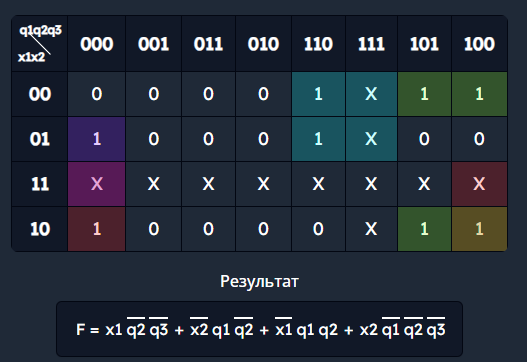
\includegraphics[scale=0.45]{img/Q1.png}
		\caption{Минимизация $Q_1$}
	\end{minipage}
	\hfill
	\begin{minipage}{0.3\textwidth}
		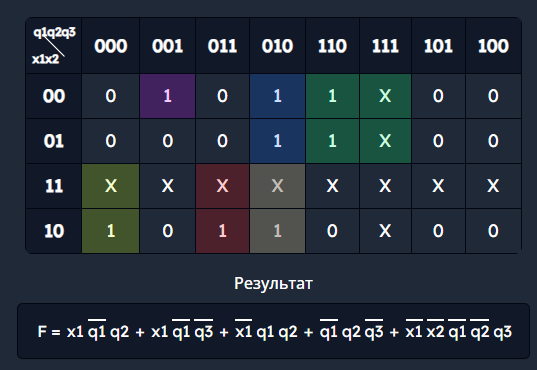
\includegraphics[scale=0.45]{img/Q2.png}
		\caption{Минимизация $Q_2$}
	\end{minipage}
	\hfill
	\begin{minipage}{0.3\textwidth}
		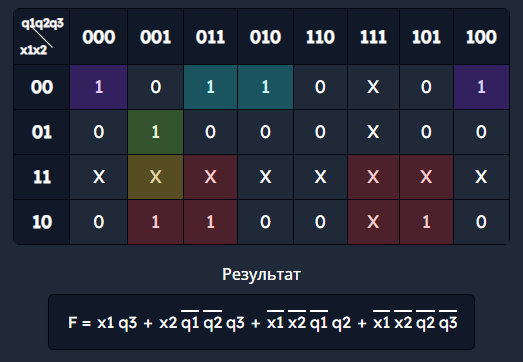
\includegraphics[scale=0.45]{img/Q3.png}
		\caption{Минимизация $Q_3$}
	\end{minipage}
	\label{Q} 
\end{figure}


\subsubsection{Минимизация L}
На \hyperref[L]{рисунках 5-10} изображена минимизация потенциальных управляющих сигналов $L_1 - L_6$ состояний конечного автомата при помощи Карты Карно.

\begin{figure}[htpb]
	\centering
	\begin{minipage}{0.25\textwidth}
		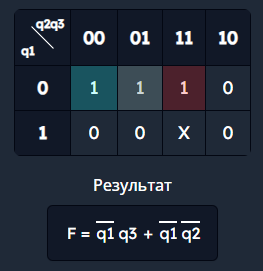
\includegraphics[scale=0.7]{img/L1.png}
		\caption{Минимизация $L_1$}
	\end{minipage}
	\hfill
	\begin{minipage}{0.25\textwidth}
		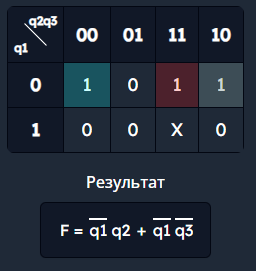
\includegraphics[scale=0.7]{img/L2.png}
		\caption{Минимизация $L_2$}
	\end{minipage}
	\hfill
	\begin{minipage}{0.25\textwidth}
		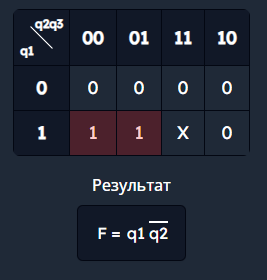
\includegraphics[scale=0.7]{img/L3.png}
		\caption{Минимизация $L_3$}
	\end{minipage}
	\hfill
	\begin{minipage}{0.25\textwidth}
		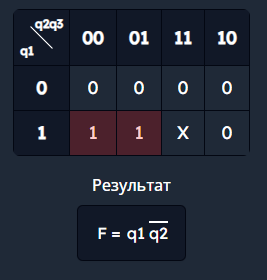
\includegraphics[scale=0.7]{img/L3.png}
		\caption{Минимизация $L_4$}
	\end{minipage}
	\hfill
	\begin{minipage}{0.25\textwidth}
		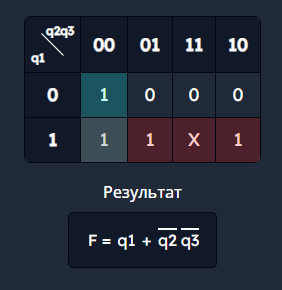
\includegraphics[scale=0.7]{img/L5.png}
		\caption{Минимизация $L_5$}
	\end{minipage}
	\hfill
	\begin{minipage}{0.25\textwidth}
		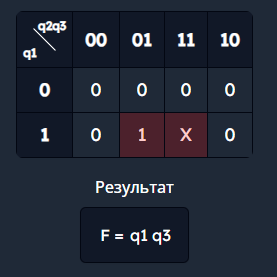
\includegraphics[scale=0.7]{img/L6.png}
		\caption{Минимизация $L_6$}
	\end{minipage}
	\label{L} 
\end{figure}

\subsubsection{Минимизация i}
На \hyperref[i]{рисунках 11-13} изображена минимизация импульсных управляющих сигналов $i_1 - i_3$  при помощи Карты Карно.

\newpage
\begin{figure}[htpb]
	\centering
	\begin{minipage}{0.3\textwidth}
		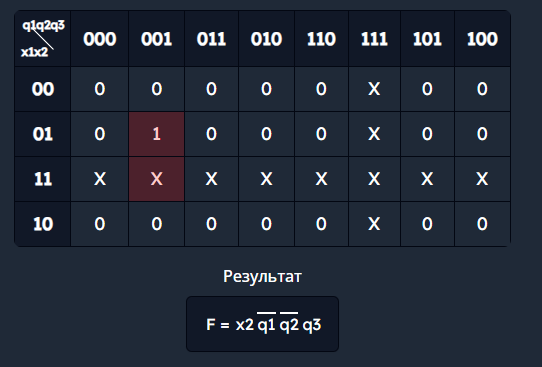
\includegraphics[scale=0.45]{img/i1.png}
		\caption{Минимизация $i_1$}
	\end{minipage}
	\hfill
	\begin{minipage}{0.3\textwidth}
		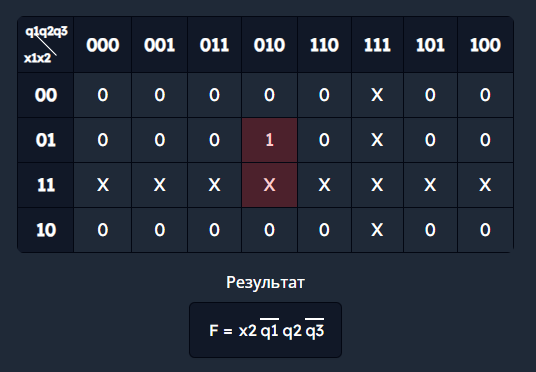
\includegraphics[scale=0.45]{img/i2.png}
		\caption{Минимизация $i_2$}
	\end{minipage}
	\hfill
	\begin{minipage}{0.3\textwidth}
		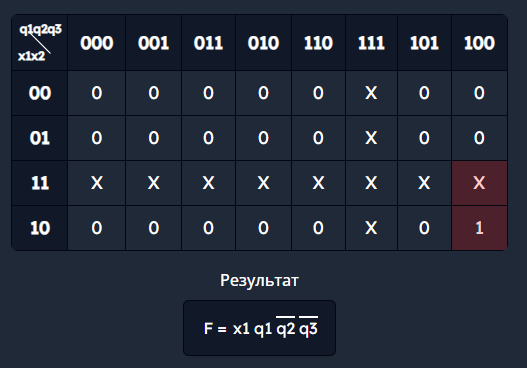
\includegraphics[scale=0.45]{img/i3.png}
		\caption{Минимизация $i_3$}
	\end{minipage}
	\label{i} 
\end{figure}



\newpage
\section{Особенности реализации}
\subsection{Анализ схемотехнических элементов}
\subsubsection{Индикаторный преобразователь}
Для отображения чисел используются  индикаторы, содержащие семь сегментов, которые, высвечиваясь в определенной комбинации, могут 
дать изображение цифры (см. \hyperref[indicator]{рис. 14}).  Для того чтобы сегмент “загорелся”, на него необходимо подать напряжение. Один разряд индикатора, таким образом, содержит 7 входов. Если на некоторые из этих входов подадим напряжение, а на остальные – нет, то на индикаторе высветится соответствующая комбинация сегментов. Например \hyperref[digit2]{(рис. 15)}, для изображения цифры <<2>> необходимо подать напряжение на все сегменты, кроме f1 и f4. 

Функциональный преобразователь, который по двоичному 
коду десятичной цифры вырабатывает сигналы, управляющие индикаторами называется индикаторный преобразователь (ИП). Его условное изображение дано на  \hyperref[IC]{рис. 16}. 

\begin{figure}[htpb]
	\centering
	\begin{minipage}{0.45\textwidth}
		\centering
		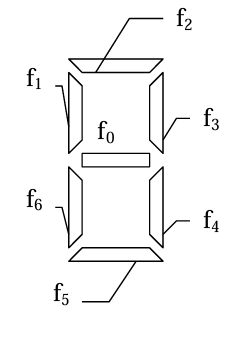
\includegraphics[scale=0.6]{img/indicator.png}
		\caption{Семисегментный индикатор}
		\label{indicator}
	\end{minipage}
	\hfill
	\begin{minipage}{0.45\textwidth}
		\centering
		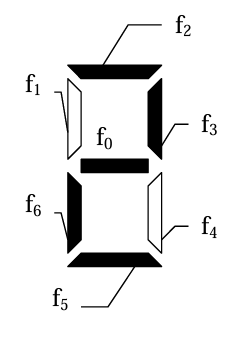
\includegraphics[scale=0.6]{img/digit2.png}
		\caption{Изображение цифры <<2>>}
		\label{digit2}
	\end{minipage}
	\hfill
	\begin{minipage}{0.9\textwidth}
		\centering
		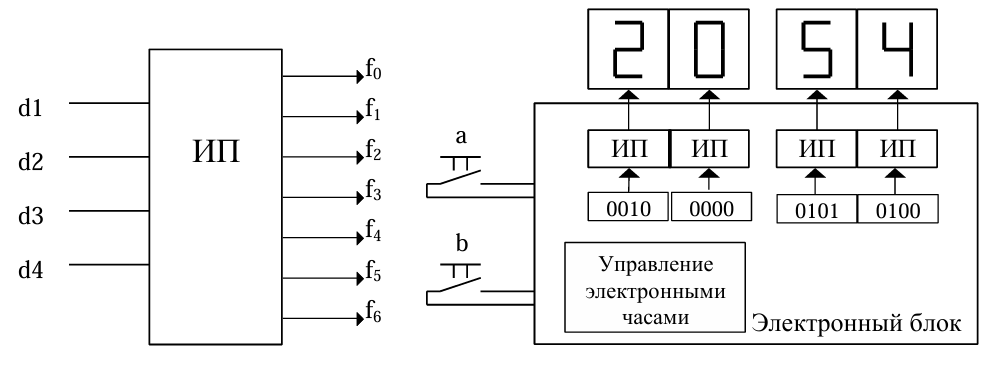
\includegraphics[scale=0.6]{img/IC.png}
		\caption{Индикаторный преобразователь}
		\label{IC}
	\end{minipage} 
\end{figure}

 Схема индикаторного преобразователя представлена на \hyperref[IC_ready]{рисунке 17}.
 
 \begin{figure}[htpb]
 	\centering
 	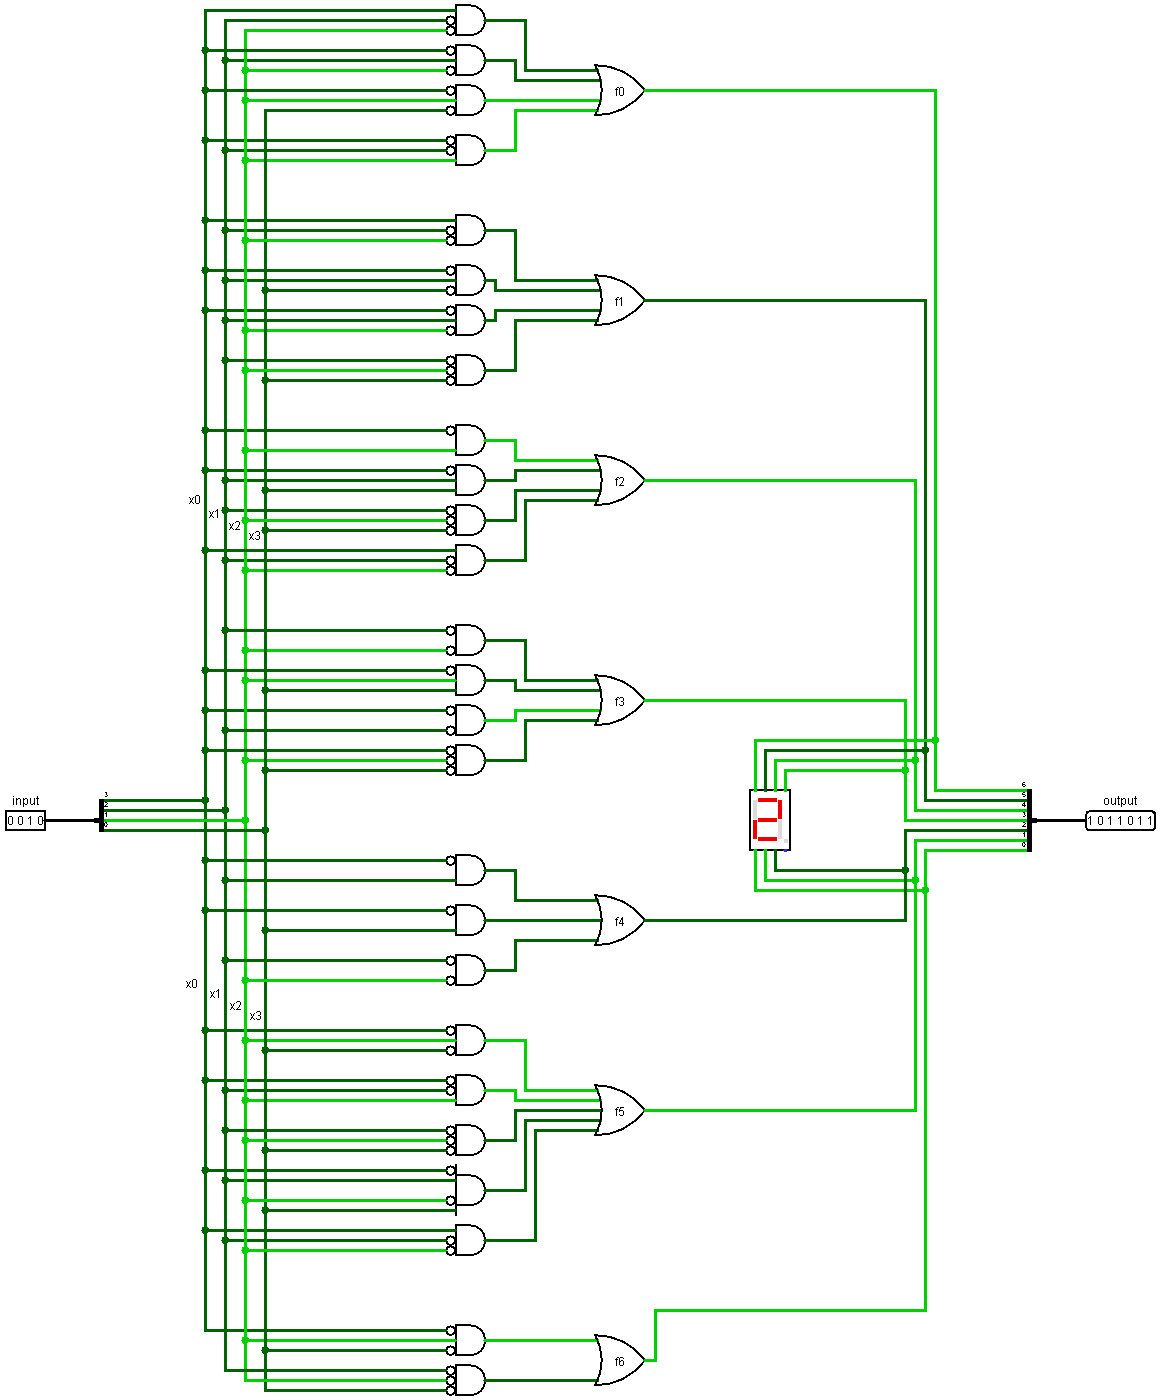
\includegraphics[scale=0.4]{logisim/img/IC.png}
 	\label{IC_ready} 
 	\caption{Схема индикаторного преобразователя}
 \end{figure}
 
\newpage
\subsubsection{Тактовый генератор}
Тактовый генератор (или генератор тактовых импульсов) — это электронное устройство, которое создает периодические электрические импульсы (такты), используемые для синхронизации работы различных компонентов электронных устройств. 

В электронных часах применяют малогабаритные стабильные генераторы, с выхода которых снимается последовательность прямоугольных импульсов. Частота кварцевых генераторов стабильна, она практически не изменяется во времени. Понятно, что количество импульсов, выработанных таким генератором, прямо пропорционально времени его работы.
\subsubsection{Счетчик}

Для реализации функции отсчета времени используются счетчики, управляемые генератором тактовых импульсов. 

Счетчик - это устройство, которое осуществляет счет и хранение кода числа подсчитанных импульсов. У каждого счетчика есть тактовый вход, на который поступают электрические импульсы, и несколько выходов, с которых можно снимать двоичный код числа, находящийся в счетчике. С каждым новым входным импульсом этот код увеличивается на 1.

Важным параметром счетчика является коэффициент пересчета К. К - это максимальное число импульсов, которое может быть подсчитано. Если рассматривать счетчик как конечный автомат, то К - это количество 
различных состояний счетчика. Счетчик с коэффициентом пересчета К через К переключений возвращается в исходное состояние. Для удобства использования счетчика, кроме тактового входа существует вход <<Уст.0>> (сброс). При подаче на него импульса (логической единицы) на выходе устанавливается нулевой код.

В качестве примера рассмотрим систему счетчиков для отсчета секунд. В первый счетчик с К=10 подаем на его вход импульсы с частотой 1 Гц с помощью генератора, также выходной сигнал, передающийся себе на сброс, подаем на вход второго генератора с К=6. Теперь когда у первого счетчика набирается 10, значение сбрасывается и на втором счетчике прибавляется единица. 

Пример системы счетчиков для отчета секунд изображен на \hyperref[counters]{рисунке 18}.

 \begin{figure}[htpb]
	\centering
	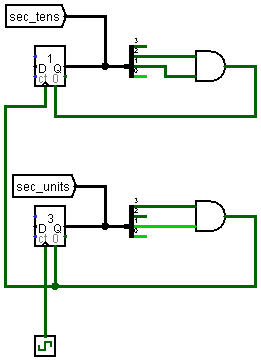
\includegraphics[scale=0.4]{logisim/img/counters.png}
	\label{counters} 
	\caption{Схема счетчиков для отсчета секунд}
\end{figure}

\subsubsection{D-триггер}
Триггер -- устройство с двумя устойчивыми состояниями. Основная его функция - хранить один бит информации неограниченное время до тех пор, пока эта информация не будет изменена воздействием на вход триггера. Существует довольно много разновидностей триггеров, различающихся по входным условиям смены состояния. 

D-триггер имеет два основных входа:
\begin{enumerate}
	\item D (Data) — данные, которые будут записаны в триггер.
	\item CLK (Clock) — тактовый сигнал, который управляет процессом записи.
\end{enumerate}

Также у него есть два выхода:
\begin{enumerate}
	\item Q — выход, который отражает текущее состояние триггера (хранит данные).
	\item $\overline{\text{Q}}$ — инвертированное состояние выхода Q.
\end{enumerate}


Микросхема D-триггера изображена на \hyperref[D-trigger]{рисунке 19}.

\begin{figure}[htpb]
	\centering
	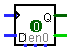
\includegraphics[scale=0.8]{logisim/img/D-trigger.png}
	\label{D-trigger} 
	\caption{Микросхема D-триггера}
\end{figure}

\subsubsection{Блок F}
Блок F предназначен для вычисления следующего состояния на основе текущего состояния и входных данных (кнопок). Помимо следующего состояния вычисляются  импульсные сигналы необходимы при переходе в следующее состояние.

Схема блока F представлена на \hyperref[F-block]{рисунке 20}.

\begin{figure}[htpb]
	\centering
	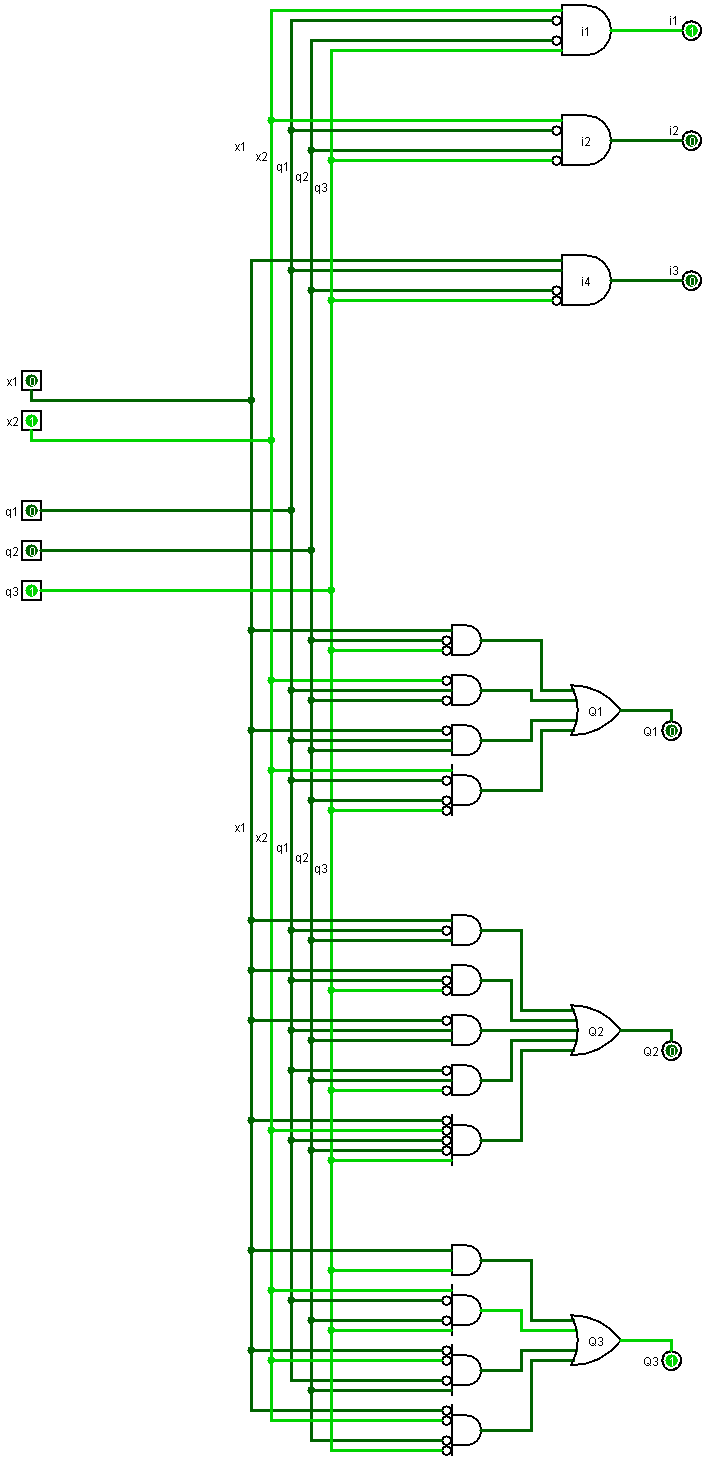
\includegraphics[scale=0.4]{logisim/img/F.png}
	\label{F-block} 
	\caption{Схема блока F}
\end{figure}

\newpage
\subsubsection{Блок памяти}
Блок памяти предназначен для хранения текущего состояния автомата. Схема блока памяти изображена на \hyperref[memory]{рисунке 21}.
\begin{figure}[htpb]
	\centering
	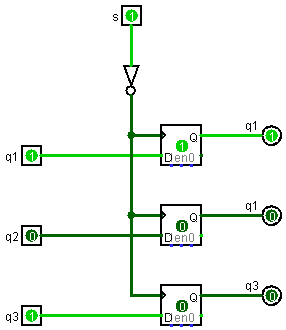
\includegraphics[scale=0.4]{logisim/img/memory.png}
	\label{memory} 
	\caption{Схема блока памяти}
\end{figure}



\subsubsection{Блок FL}
Блок FL отвечает за формирование потенциальных сигналов на основе  текущего состояния автомата. Схема блока FL представлена на \hyperref[FL-block]{рисунке 22}.
\begin{figure}[htpb]
	\centering
	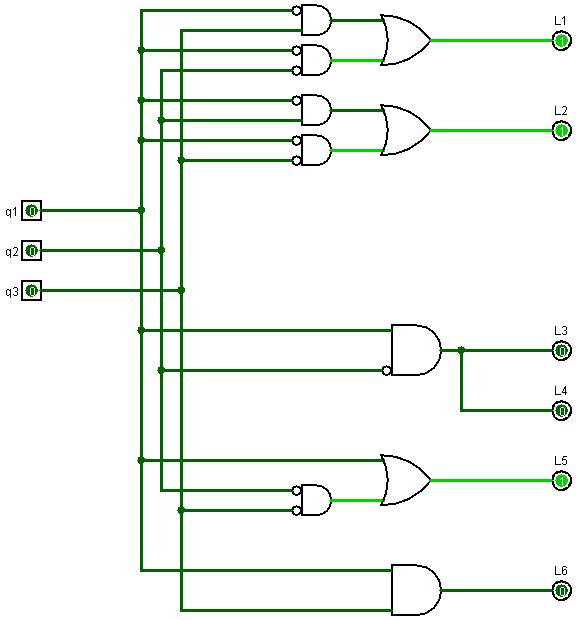
\includegraphics[scale=0.4]{logisim/img/FL.png}
	\label{FL-block} 
	\caption{Схема блока FL}
\end{figure}

\subsubsection{Преобразователь внешних воздействий}
Данный блок предназначен для конвертации нажатой кнопки в соответствующие сигналы $x_0$ и $x_1$. Также он создает синхроимпульс, который необходим для работы в блоке памяти.
Схема преобразователя внешних воздействий изображена на \hyperref[BC]{рисунке 23}.
\begin{figure}[htpb]
	\centering
	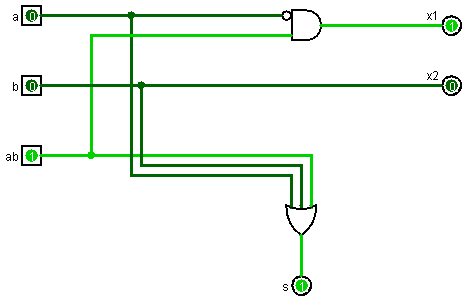
\includegraphics[scale=0.4]{logisim/img/BC.png}
	\label{BC} 
	\caption{Схема блока FL}
\end{figure}

\subsubsection{Машина состояний}
Данная схема представляет машину состояний или конечный автомат электронных часов. Она предназначена для переключения состояний в зависимости от входных сигналов. Она состоит из блоков F, FL и блока памяти.

Схема конечного автомата часов представлена на \hyperref[state machine]{рисунке 24}.
\begin{figure}[htpb]
	\centering
	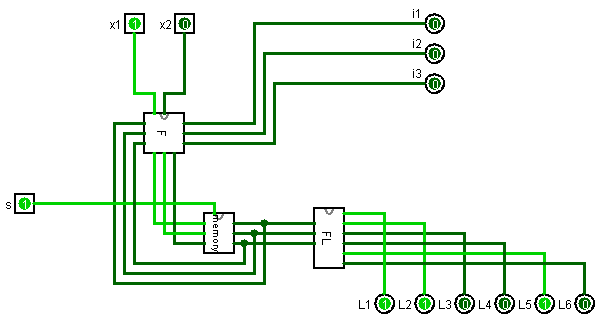
\includegraphics[scale=0.4]{logisim/img/state machine.png}
	\label{state machine} 
	\caption{Схема конечного автомата часов }
\end{figure}


\subsubsection{Отсчет времени часов}
Данная схема предназначена для отсчета времени часов. Она состоит из системы счетчиков.  
Схема отсчета времени у часов представлена на \hyperref[clock]{рисунке 25}.
\newpage
\begin{figure}[htpb]
	\centering
	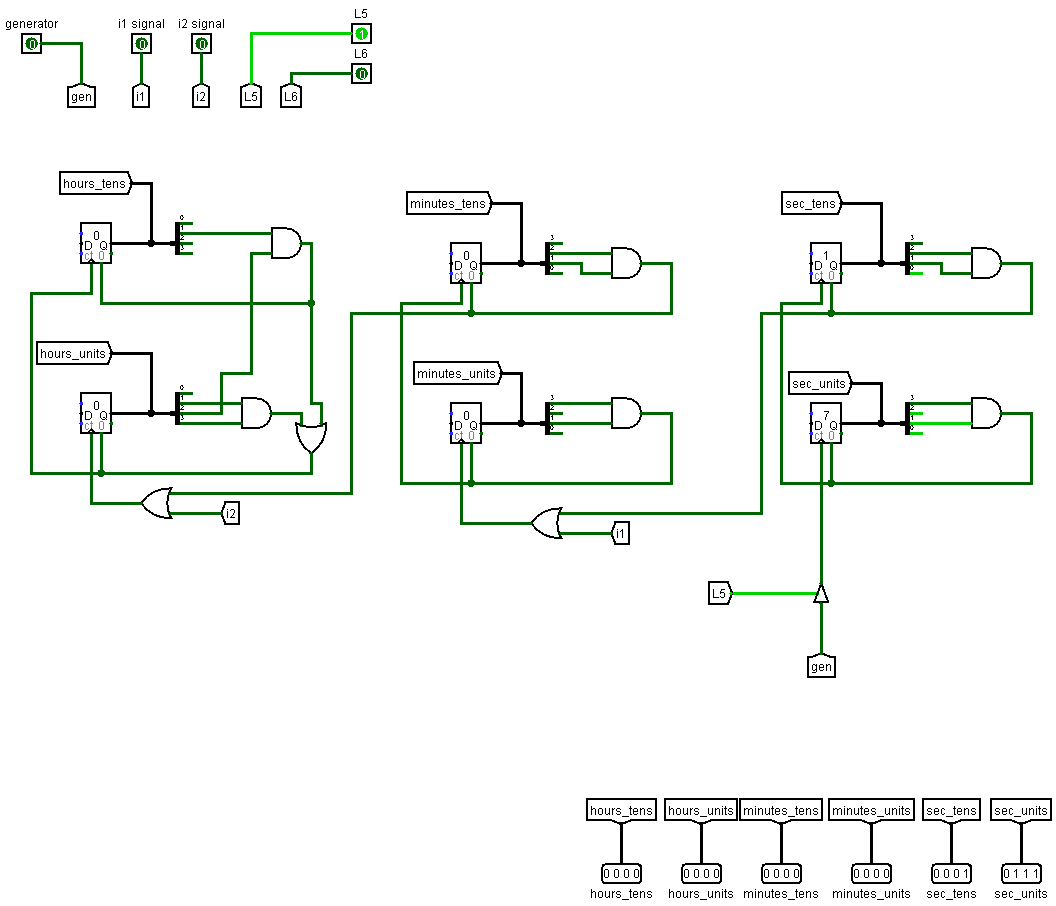
\includegraphics[scale=0.4]{logisim/img/clock.png}
	\label{clock} 
	\caption{Схема отсчета времени часов }
\end{figure}


\subsubsection{Отсчет времени секундомера}
Данная схема предназначена для отсчета времени секундомера. Она состоит из системы счетчиков.  
Схема отсчета времени у секундомера представлена на \hyperref[SW]{рисунке 25}.
\newpage
\begin{figure}[htpb]
	\centering
	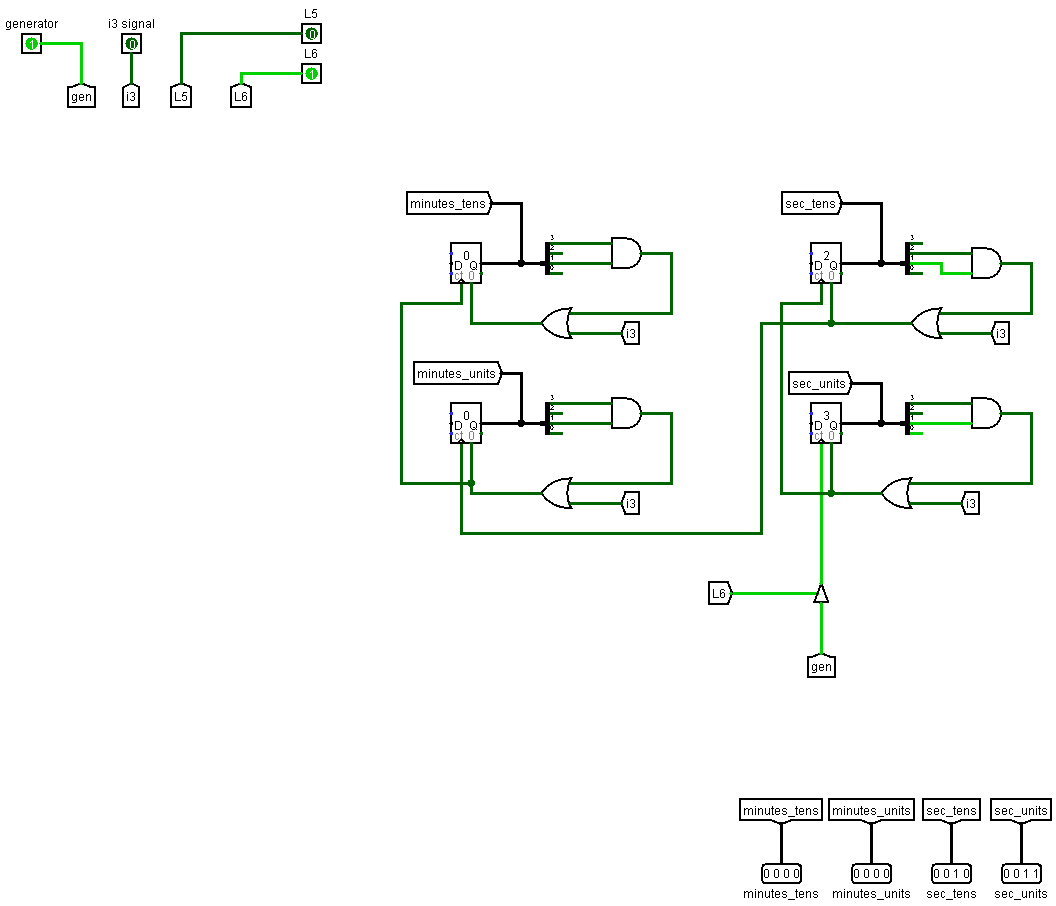
\includegraphics[scale=0.4]{logisim/img/SW.png}
	\label{SW} 
	\caption{Схема отсчета времени секундомера }
\end{figure}

\subsubsection{Звуковая сигнализация}
Так как в Logisim нет звукового выхода, имитация звуковой сигнализации происходит с помощью светодиода.
В данной схеме происходит сохранения выходного сигнала каждую четверть часа в течении секунды с помощью D-триггера и счетчика. 
Схема звуковой сигнализации изображена на  \hyperref[signal]{рисунке 26}.
\newpage
\begin{figure}[htpb]
	\centering
	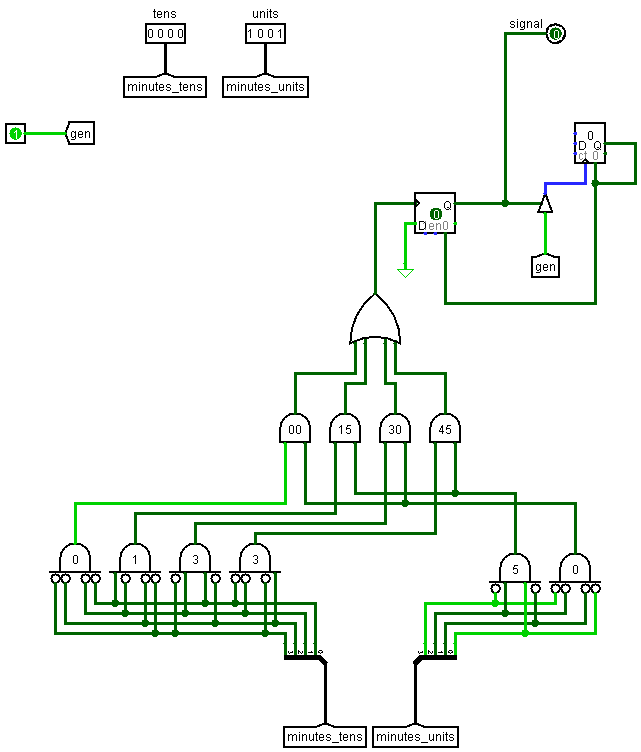
\includegraphics[scale=0.4]{logisim/img/signal.png}
	\label{signal} 
	\caption{Схема звуковой сигнализации }
\end{figure}

\subsubsection{Интерфейс часов}
Интерфейс часов состоит из 4 индикаторов, отображающих часы и минуты текущего времени, а также минуты и секунды секундомера. Для управления часами присутствуют кнопки <<а>>, <<b>> и кнопка, имитирующая одновременное их нажатие, <<ab>>.

Схема интерфейса электронных часов изображена на \hyperref[main]{рисунке 27}.
\newpage
\begin{figure}[htpb]
	\centering
	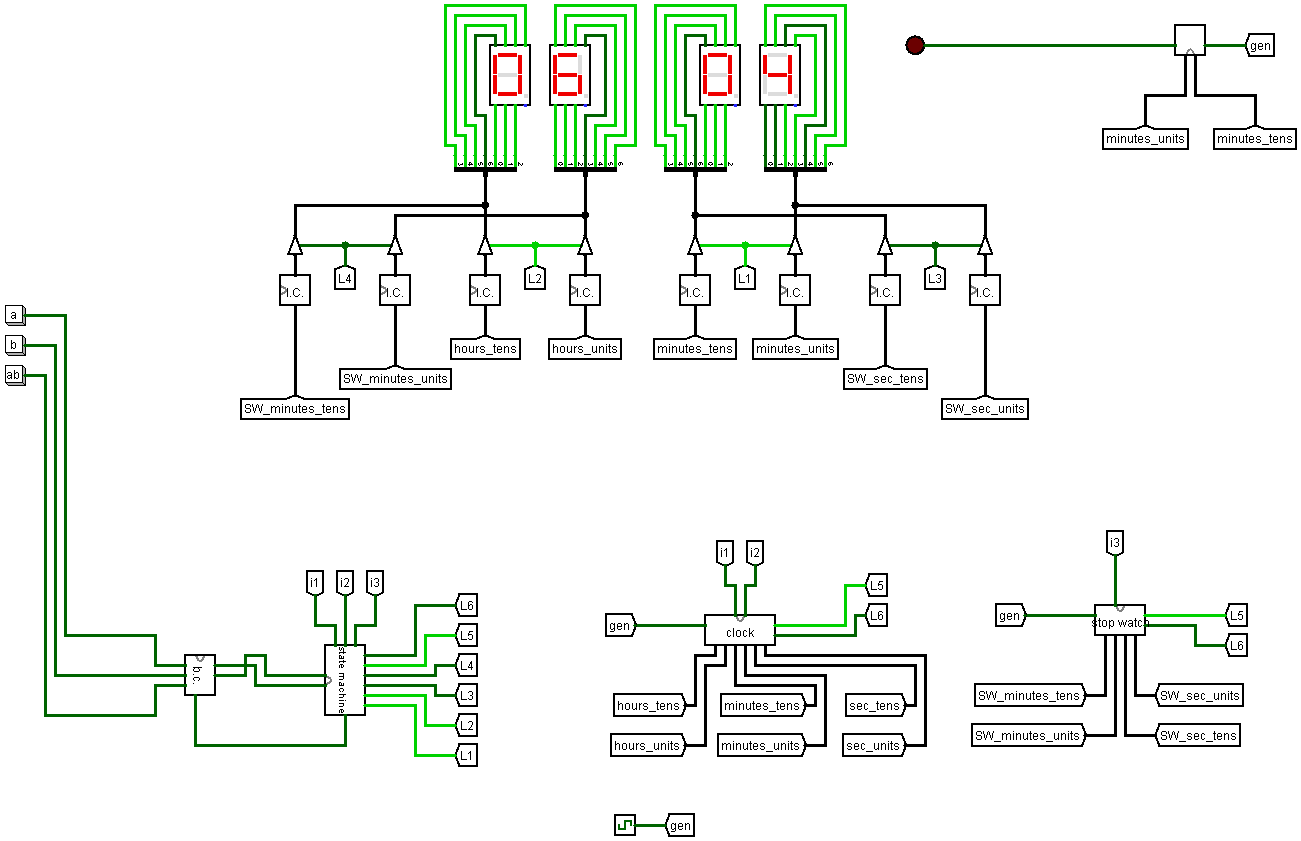
\includegraphics[scale=0.35]{logisim/img/main.png}
	\label{main} 
	\caption{Схема интерфейса электронных часов}
\end{figure}


\subsection{Расчет площади схемы}
Количество компонентов каждого типа на функциональной функциональной схеме электронных часов отображено на \hyperref[statistic]{рисунке 27}.
\newpage
\begin{figure}[htpb]
	\centering
	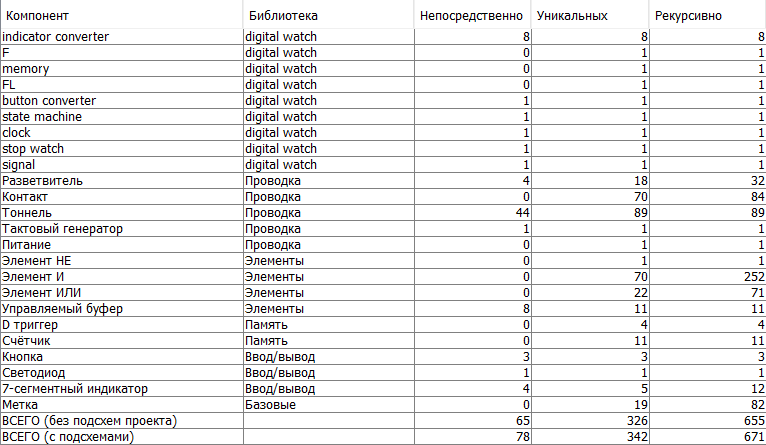
\includegraphics[scale=1]{logisim/img/statistic.png}
	\label{statistic} 
	\caption{Статистика функциональной схемы часов}
\end{figure}

\begin{enumerate}[label=]
	\item Непосредственно -- количество компонентов, которые напрямую размещены на главной схеме. Если схема использует вложенные подсхемы, то количество их компонентов не подсчитывается.
	\item Уникальных -- общее количество уникальных компонентов одного типа, включая те что находятся внутри подсхем. Если подсхема используется несколько раз, то компоненты в ней считаются всего один раз.
	\item Рекурсивно -- полное количество компонентов, включая все из подсхем. Учитываются все экземпляры дублирующихся подсхем.
\end{enumerate}

Рассчитаем число транзисторов для каждого компонента с учетом количества его вхождений в схему.
\begin{enumerate}[label=]
	\item $\text{Инвертор: } 4 * 1 = 4$ 
	\item $\text{И: }  6 * 252 = 1512$
	\item $\text{ИЛИ: }  4 * 71 = 284$
	\item $\text{Управляемый буфер: }  4 * 11 = 44$
	\item $\text{D-триггер: }  20 * 4 = 80$
	\item $\text{Счетчик: }  16 * 2 * 10 + 16 * 1 * 1 = 336$
	\item $\text{7-сегментный индикатор: }  7 * 17 = 119$
	\item Другие компоненты не требуют транзисторов.
\end{enumerate}
Итого получается  $2379$ транзисторов на данную функциональную схему. Исходя из расчета, что на 1 $mm^2$ приходится примерно 1000 транзисторов, функциональная схема реализованных часов будет занимать примерно $2,379mm^2$


\newpage
\addcontentsline{toc}{section}{Заключение}
\section*{Заключение}
В ходе выполнения курсовой работы была разработана функциональная схема электронных часов, реализующих следующие функции:
\begin{itemize}
	\item Отображение и корректировка минут, часов.
	\item 24-часовой формат времени.
	\item Отключение индикаторов с целью экономии электроэнергии.
	\item Останов часов после состояния корректировки текущего времени.
	\item Секундомер с фиксацией накопленного времени и возможностью продолжения отсчета секундомера.
	\item Звуковая сигнализация каждые четверть часа в течение секунды.
\end{itemize}
Преимущества реализованной функциональной схемы часов:
\begin{enumerate}
	\item При минимизации функций блоков FL, F и i-формирователя использовалась недоопределённость частичных функций.
	\item Наличие отключения/включения индикаторов во время корректировки времени.
\end{enumerate}
Недостатки реализованной функциональной схемы часов:
\begin{enumerate}
	\item Наличие лишнего сигнала $L_4$, отвечающий за отображение минут у секундомера. В функционале часов у секундомера не бывает что минуты и секунды отображаются отдельно, поэтому было бы достаточно всего одного сигнала $L_3$, который отвечал бы не только за отображение секунд, но и минут.
	\item Недостаточно хорошо разработан граф конечного автомата: во время нажатия кнопки <<ab>>, можно было бы сделать сброс накопленного времени с переходом в состояния остановленного секундомера.
\end{enumerate}
Масштабирование: к реализованной функциональной схеме часов можно добавить отображение секунд, дня недели или день месяца. Также можно добавить будильник.\\

\noindent Функциональная схема электронных часов была реализована в Logisim 2.7.1. 

\newpage
\addcontentsline{toc}{section}{Список литературы}

\begin{thebibliography}{0}
	\bibitem{tema} Методические указания к курсовой работе. Сайт секции <<Телематика>>. - Текст: электронный // tema.spbstu.ru : [сайт]. - URL: \href{https://tema.spbstu.ru/userfiles/files/courses/2018-theory-algorithm/KuR\_MU.pdf}{https://tema.spbstu.ru/userfiles/files/courses/2018-theory-algorithm/KuR\_MU.pdf} (дата обращения 01.11.2024).
	\bibitem{karpov}  Карпов Ю. Г. Теория автоматов. Питер, 2003 г., 206 с.
	\bibitem{Ericson} Эриксон Д. Алгоритмы. ДМК-Пресс, 2023 г., 526 с.
\end{thebibliography}

\end{document}
